%%%%%%%%%%%%%%%%%%%%%%%%%%%%%%%%%%%%%%%%
% Load the document template. 
\documentclass{report}

%%%%%%%%%%%%%%%%%%%%%%%%%%%%%%%%%%%%%%%%
% By default, the template loads several 
% packages you are likely to need or that 
% were required to format the document: 
    % geometry, calc, hyperref, mathptmx, amsmath,
    % mhchem, inputenc, graphicx, setspace, titlesec,
    % fancyhdr, biblatex
% Other packages can be loaded as:
\usepackage{lipsum}

%%%%%%%%%%%%%%%%%%%%%%%%%%%%%%%%%%%%%%%%
% Tells you which file containts the bibtex 
\addbibresource{refs.bib}


%%%%%%%%%%%%%%%%%%%%%%%%%%%%%%%%%%%%%%%%
% Insert some required information here.
\title{Summary of Research Progress:\\A \LaTeX\ Template to Help You With Your Quals}
\author{Your Name}
\lab{Professor Sandy Cheeks Research Laboratory}
\department{Department of Chemistry, Massachusetts Institute of Technology, Cambridge, MA, USA}
% You can simply replace \today with the date of your oral.
\date{\today}

%%%%%%%%%%%%%%%%%%%%%%%%%%%%%%%%%%%%%%%%
% This makes the above definitions values callable 
% in the report.cls file. Leave it be. 
\makeatletter

%%%%%%%%%%%%%%%%%%%%%%%%%%%%%%%%%%%%%%%%
% Set pdf information. Be sure to replace
% the PDF title with the correct information. 
\hypersetup{
    pdfsubject = {Qualifying Exam Written Report: \@author},
    pdftitle = {Lastname-Firstname-Year.pdf},
    pdfauthor = {\@author},
    colorlinks=true,
    linkcolor=black,
    filecolor=magenta,
    urlcolor=cyan,
    citecolor=black
}

%%%%%%%%%%%%%%%%%%%%%%%%%%%%%%%%%%%%%%%%
% Begin document
%%%%%%%%%%%%%%%%%%%%%%%%%%%%%%%%%%%%%%%%
\begin{document}

% Print the formatted title, name, affiliations, date. 
\maketitle

% Create a bookmark in the PDF for each of the sections
\pdfbookmark[section]{\contentsname}{toc}

% Force the page number of the first page to the bottom right.
% Without this, the fancy pagestyle starts on the second page.
\thispagestyle{fancy}


%%%%%%%%%%%%%%%%%%%%%%%%%%%%%%%%%%%%%%%%
% Write each section in the specified file in the sections folder. 
% Placing different information in the different files
% makes it easier to independently save multiple versions of each section, 
% replace them, rearrange them, etc., rather than always needing to
% modify the master. 
% The example text contained in the pdf, for example, can be removed by deleting the following two lines. 
\section{Some Simple Commands}
The text you're reading is contained in the sections/0\_example\_uses.tex file. 
Separating 
words, 
phrases, 
sentences, 
etc.
by 
a 
newline 
continues
the 
same 
paragraph. 

Instead, separate text by two newlines to start a new paragraph.

\begin{figure}[H] % The H demands that the figure appear at this point in the text
    \centering
    % The graphics will be 20 percent of the width of the text. 
    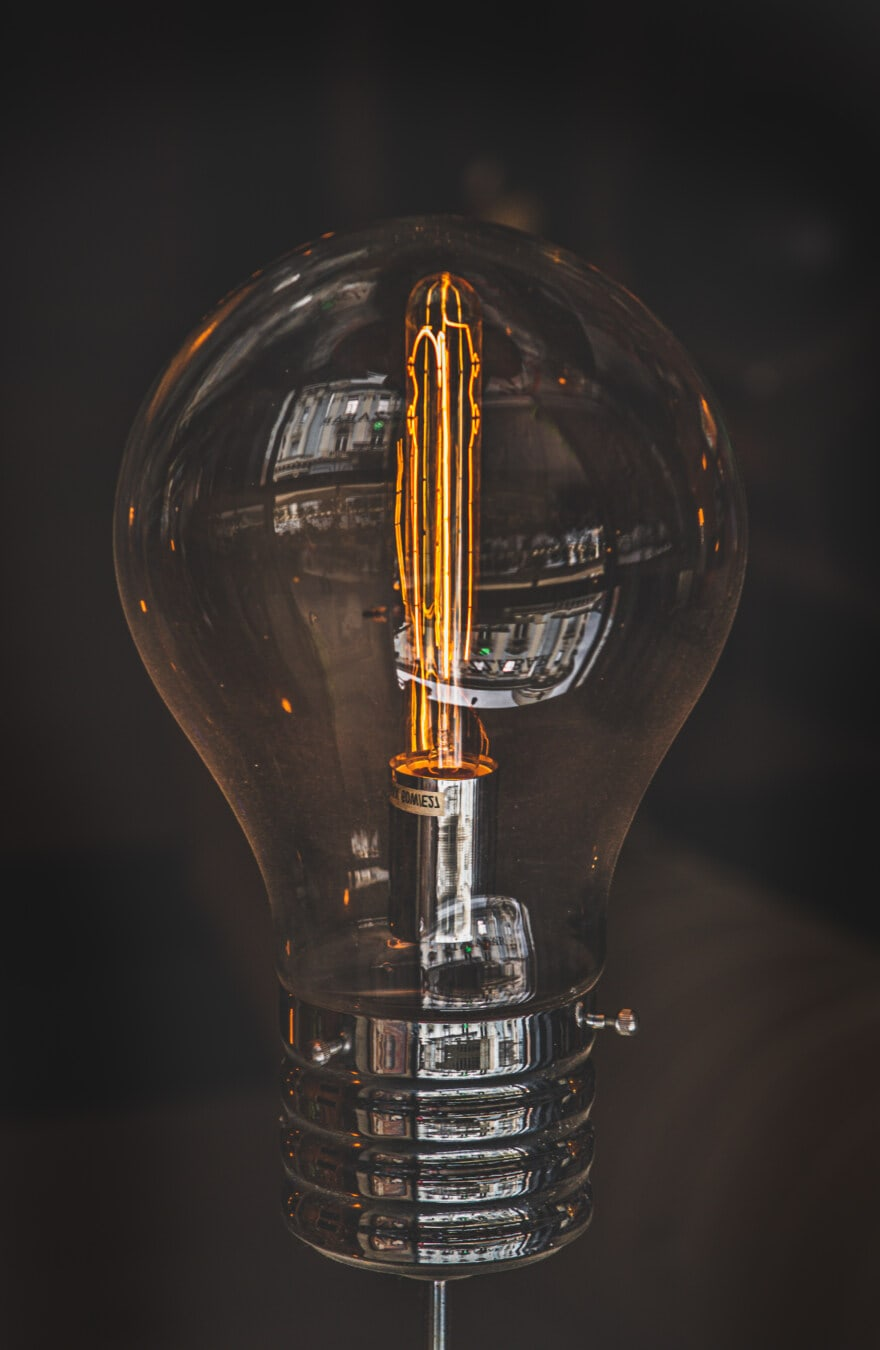
\includegraphics[width=0.2\textwidth]{figures/lightbulb.jpeg}
    \caption{
    \textbf{This is the top hit for ``science'' on \href{https://pixnio.com/?s=science}{pixnio}.} (They provide free images!)
    }
    \label{fig:figure_name}
\end{figure}

% The figure takes up 30 percent of the page width used by text.
\begin{wrapfigure}{l}{0.3\textwidth}
    \begin{center} 
        % The image takes up 20 percent of the page width used by text.
        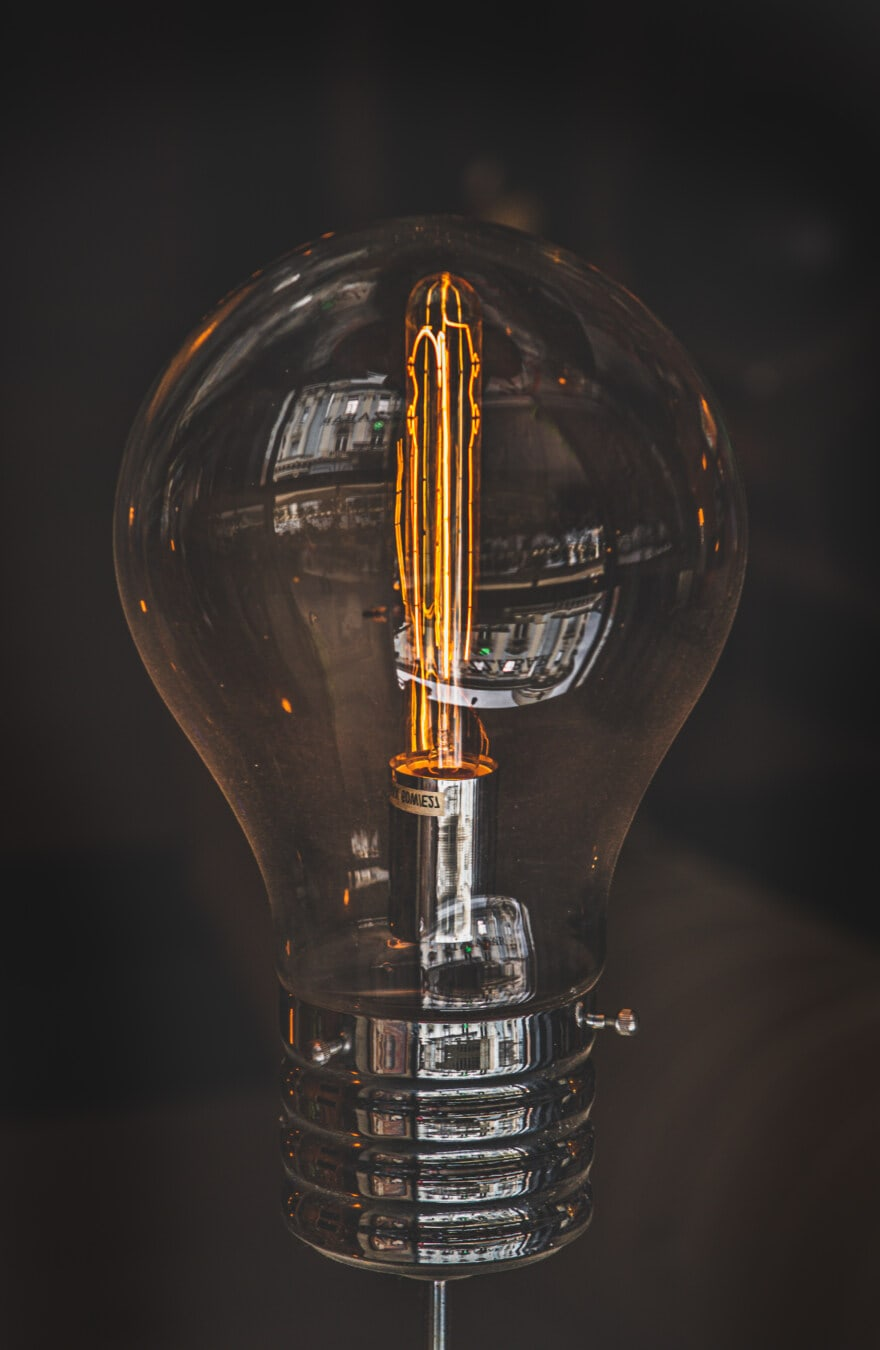
\includegraphics[width=0.2\textwidth]{figures/lightbulb.jpeg}
    \end{center}
    \caption{I guess Edison's work \textit{does} outshine mine\ldots }
    \label{fig:wrapped_figure}
\end{wrapfigure}
Formatting is generally easiest if you include figures with the \textbackslash begin\{figure\} command, as in Fig.~\ref{fig:figure_name}. However, as with Fig.~\ref{fig:wrapped_figure}, you can save space by wrapping text around figures with the wrapfig package. More details about using wrapfig are available \href{https://www.overleaf.com/learn/latex/Wrapping_text_around_figures}{here}. Captions number correctly regardless of your chosen command. 
 
When formatting text, \textbackslash textit\{\} \textit{italicizes} text, \textbackslash textbf\{\} \textbf{bolds} text, and \textbackslash underline\{\} \underline{underlines} text. For more information, overleaf has many high-quality tutorials \href{https://www.overleaf.com/learn/latex/Tutorials}{here}, and the answer to nearly any \LaTeX\ question can be googled. (Oh yeah, the hyperref package provided that hyperlink functionality via \textbackslash href\{\}\{\}.)  

Equations are written like
\begin{equation}
    \label{eq:equation_name}
    E = mc^2, 
\end{equation}
and the amsmath (American Math Society) style is used to format equations in the template. Alternatively, math can be written in-text like so: $E=mc^2$. 

Chemical equations are easy to include thanks to the mhchem package. 
\begin{equation}
    \label{eq:carbonic_acid_equilibrium}
    \ce{ 
    H2O + CO2 <=> H2CO3
    }
\end{equation}
If you'd prefer \textit{not} to number an equation (whether mathematical or chemical), use \$\$.
$$ \ce{ A+(aq) + B-(aq) -> AB(s) } $$

Reference sources \textit{within} the document using \textbackslash ref\{label\_defined\_in\_tex\_file\}. This can be done with multiple objects, e.g. Fig.~\ref{fig:figure_name}, Eq.~\ref{eq:equation_name}, and Section~\ref{sec:introduction}. 

Reference outside sources with \textbackslash cite\{name\_in\_refs.bib\}. Conveniently, references~\cite{youssef_scalable_2021} automatically~\cite{sood_coupling_2022} number~\cite{schuette_decorrelating_2023} according~\cite{schuette_applying_2020} to~\cite{youssef_scalable_2023} order~\cite{schuette_efficient_2023} of~\cite{zhang_topology_2015} appearance~\cite{zhang_shape_2016}. Also, if multiple citations are included at once, then sequential articles are formatted with a dash to save space, for example~\cite{sood_coupling_2022,youssef_scalable_2021,schuette_decorrelating_2023,youssef_scalable_2023,schuette_efficient_2023,zhang_topology_2015,zhang_shape_2016,schuette_applying_2020}. (Note that it also places the citations on the correct side of punctuation marks!) All of these in-text citation rules follow the \textit{J. Am. Chem. Soc.} (with title) formatting guidelines. 

You can add subsections to help break up your report. For example, Subsection~\ref{subsec:format} discusses a bit about the formatting of this document. 

\subsection{The Formatting Guidelines}
\label{subsec:format}

This document uses letter paper, which has dimensions 8.5''$\times$ 11'', and it uses 1 inch margins everywhere. All text is single-spaced with 12 point Times Roman font. Page numbers are included in the bottom right and are also shown with 12 point Times Roman font. 

In lieu of a cover page, the report's title and your name, lab, department, and oral exam date can be inserted in the header of the file main.tex, and they're displayed as in this Lastname-Firstname-Year.pdf. (Comments walk you through these steps and begin with \%.) Similarly, the file will currently save as Lastname-Firstname-Year.pdf, but you can change this to your information by modifying the text on line 39 of main.tex. Otherwise, the only change you should need to make to main.tex is deleting lines 71 and 72, which will remove this tutorial section and its associated references. 

Each section of your report should be typed in the corresponding file in the sections folder. Partitioning the information in the different files makes it easier to independently save multiple versions of each section, replace them, rearrange them, etc., rather than always needing to modify the main file. Simply remove the existing \textbackslash lipsum commands, which insert lorem ipsum text as a placeholder, and get to writing! 

Image files can be placed in the figures folder to maintain organization. Replace gantt\_chart.png in that folder with your own, which is probably easiest to make as a table in Microsoft Word. 

Place your references in refs.bib using Bib\TeX format. This can easily be done with \href{https://www.zotero.org/}{Zotero}, which will provide the Bib\TeX citation given just the DOI number. Conveniently, Zotero can be \href{https://www.overleaf.com/learn/how-to/How_to_link_your_Overleaf_account_to_Mendeley_and_Zotero}{directly linked to your Overleaf} so that the references are also directly imported, meaning you don't even need to copy/paste the references. If you do this, you'll need to change line 17 of the main text from \textbackslash addbibresource\{refs.bib\} to \textbackslash addbibresource\{refs.bib,imported\_file.bib\}. NOTE: Only bibliographic items referenced in the text via the \textbackslash cite\{\} command will appear in the bibliography at the end of the document. 





%%%%%%%%%%%%%%%%%%%%%%%%%%%%%%%%%%%%%%%%
\section{Long-Term Objective}
\label{sec:objective}
% Remove the \lipsum command, which simply generates text to help fill the template
\lipsum[1]


%%%%%%%%%%%%%%%%%%%%%%%%%%%%%%%%%%%%%%%%
\section{Introduction}
\label{sec:introduction}
Citations~\cite{youssef_scalable_2021} automatically~\cite{sood_coupling_2022} number~\cite{schuette_decorrelating_2023} according~\cite{schuette_applying_2020} to~\cite{youssef_scalable_2023} order~\cite{schuette_efficient_2023} of~\cite{zhang_topology_2015} appearance~\cite{zhang_shape_2016}.

% Remove the \lipsum command, which simply generates text to help fill the template
\lipsum[2]


%%%%%%%%%%%%%%%%%%%%%%%%%%%%%%%%%%%%%%%%
\section{Progress Report}
\label{sec:progress_report}
% Remove the \lipsum command, which simply generates text to help fill the template
\lipsum[3]

%%%%%%%%%%%%%%%%%%%%%%%%%%%%%%%%%%%%%%%%
\section{Plan for Upcoming Research}
\label{sec:plan_upcoming}
% Remove the \lipsum command, which simply generates text to help fill the template
\lipsum[4]

%%%%%%%%%%%%%%%%%%%%%%%%%%%%%%%%%%%%%%%%
\section{Gantt Chart for Future Planning}
\label{sec:gantt_chart_text}
% Remove the \lipsum command, which simply generates text to help fill the template
\lipsum[5]

%%%%%%%%%%%%%%%%%%%%%%%%%%%%%%%%%%%%%%%%
\section{Contributions and Acknowledgements}
\label{sec:contribution_acknowledgements}
% Remove the \lipsum command, which simply generates text to help fill the template
\lipsum[6]

I thank Greg Schuette for providing a \LaTeX template for this written report~\cite{schuette_template_2023}. 

%%%%%%%%%%%%%%%%%%%%%%%%%%%%%%%%%%%%%%%%
% Per the instructions, the Gantt chart can be placed on 
% a different page that doesn't count towards the total. 
\newpage
\section{Gantt Chart}
\label{sec:gantt}
\begin{center}
\begin{ganttchart}[
expand chart=\textwidth,
time slot format=isodate-yearmonth,
time slot unit=month,
newline shortcut=true,
bar/.append style={fill=mit_red, rounded corners=5pt},
bar label node/.append style=%
{align=left}
]{2024-5}{2025-4} % time range (year-month) of the gantt chart
  \label{fig:gantt}
  \gantttitlecalendar{year, month} \\

% Gantt chart content starts here
  \ganttbar{Second Year Oral and Written Exam}{2024-05}{2024-05}
  \ganttnewline[thick, mit_silvergray] % line that divides between entries
  \ganttbar{%
  Surprise Everyone in the World \ganttalignnewline
  with Ground-breaking Discoveries%
  }{2024-05}{2024-06} \\ % to break line within the gantt chart entry, decorate with percent symbol and like above
  \ganttbar{Write Manuscript}{2024-06}{2024-08}\\
  \ganttbar{Present at a Conference}{2024-08}{2024-08}
  \ganttnewline[thick, mit_silvergray]
  \ganttbar{%
  Discover a Highly Effective \ganttalignnewline
  Stock Market Prediction Model%
  }{2024-08}{2024-12}\\
  \ganttbar{Graduate Early
  }{2025-1}{2025-1}
\end{ganttchart}
\end{center}

%%%%%%%%%%%%%%%%%%%%%%%%%%%%%%%%%%%%%%%%
% Place the references on a new page
\newpage
\printbibliography


\end{document}
